\documentclass[12pt]{article}
\pagenumbering{gobble}

\usepackage{fancyhdr}
\usepackage[margin=1in]{geometry}
\usepackage{mathtools}

\begin{document}
    \pagestyle{fancy}

    \fancyhead[L]{Homework 1}
    \fancyhead[C]{Operating Systems}
    \fancyhead[R]{Alex Agruso}

    \begin{itemize}
        \item [1.)] With 100 packets per second, and 0.2ms per packet, we know
        that the CPU is interrupted for $100 \times 0.2 = 20$ milliseconds,
        thus the percentage of time spent handling packets is
        $20\text{ms} \div 1000\text{ms} = 0.02 = 2\%$.

        \item [2.)] If the new context is already loaded into one of the
        register sets, then the CPU changes the pointer that points
        to the current register set to point to the new context.
        If all register sets are in use, then the new context swaps with
        one of the register sets, and the old context is written to memory.

        \item [3.)] \begin{itemize}
            \item [a.)] \ 
            \begin{center}
                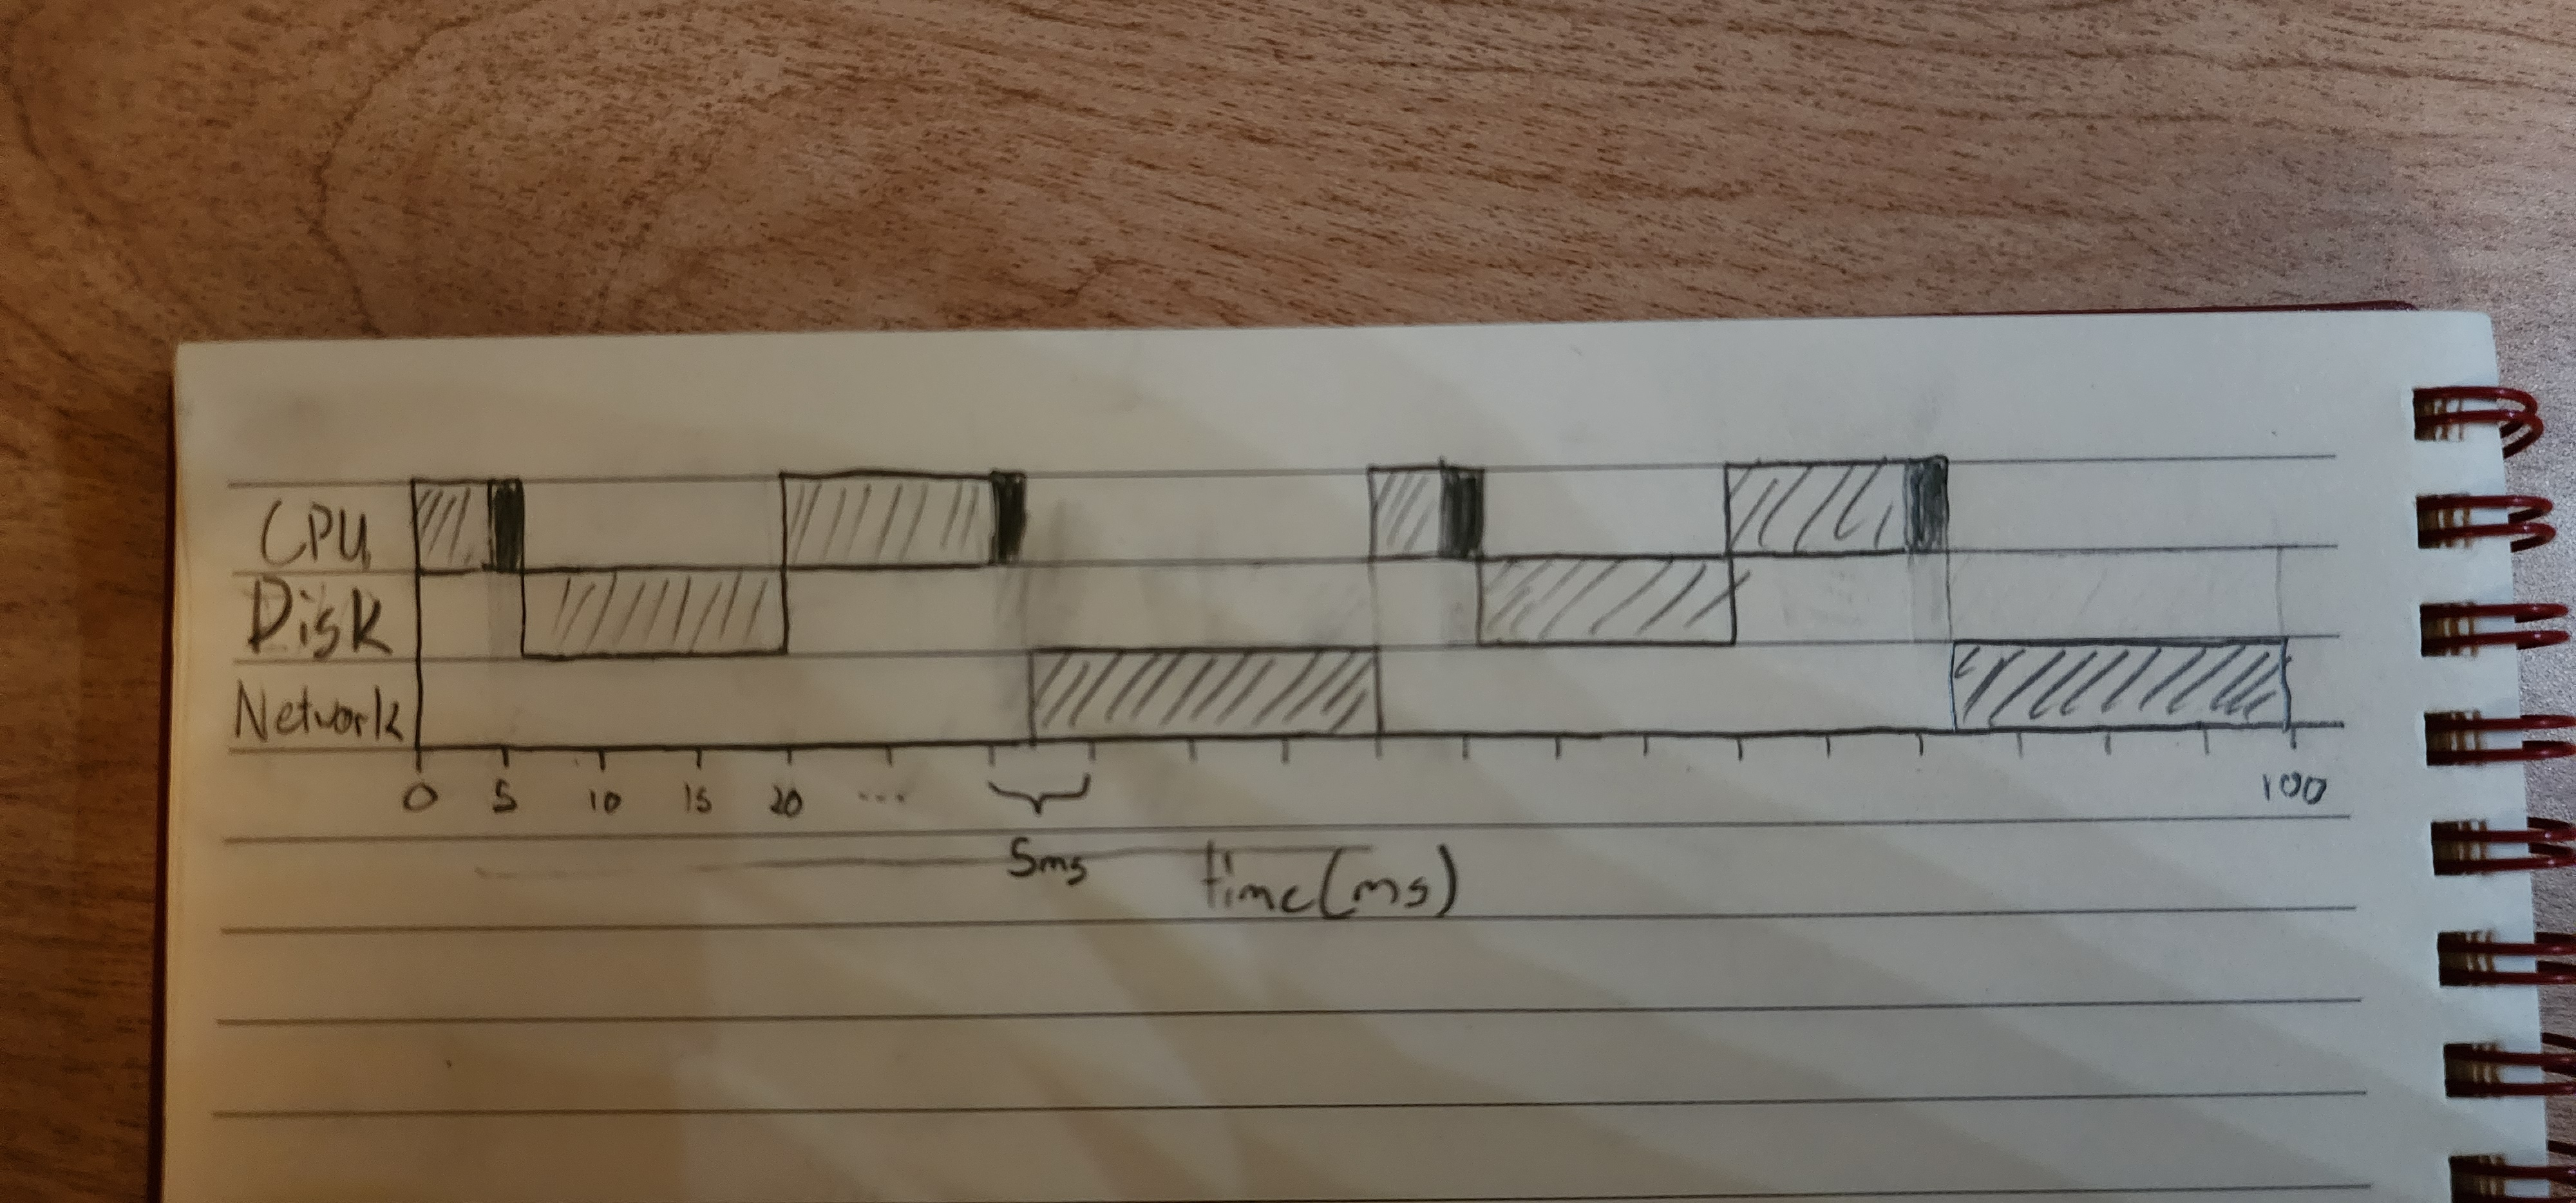
\includegraphics[width=5in]{3-1.jpg}
            \end{center}

            \item [b.)] Since it takes 100ms for the process to iterate twice,
            we can see that the average utilization of each device is
            \[
                U_{\text{CPU}}
                = \frac{2(4 + 2 + 10 + 2)}{100}
                = \frac{36}{100}
                = 36\%
            \]
            \[
                U_{\text{Disk}}
                = \frac{2(14)}{100}
                = \frac{28}{100}
                = 28\%
            \]
            \[
                U_{\text{Network}}
                = \frac{2(18)}{100}
                = \frac{36}{100}
                = 36\%
            \]

            \item [c.)] \
            \begin{center}
                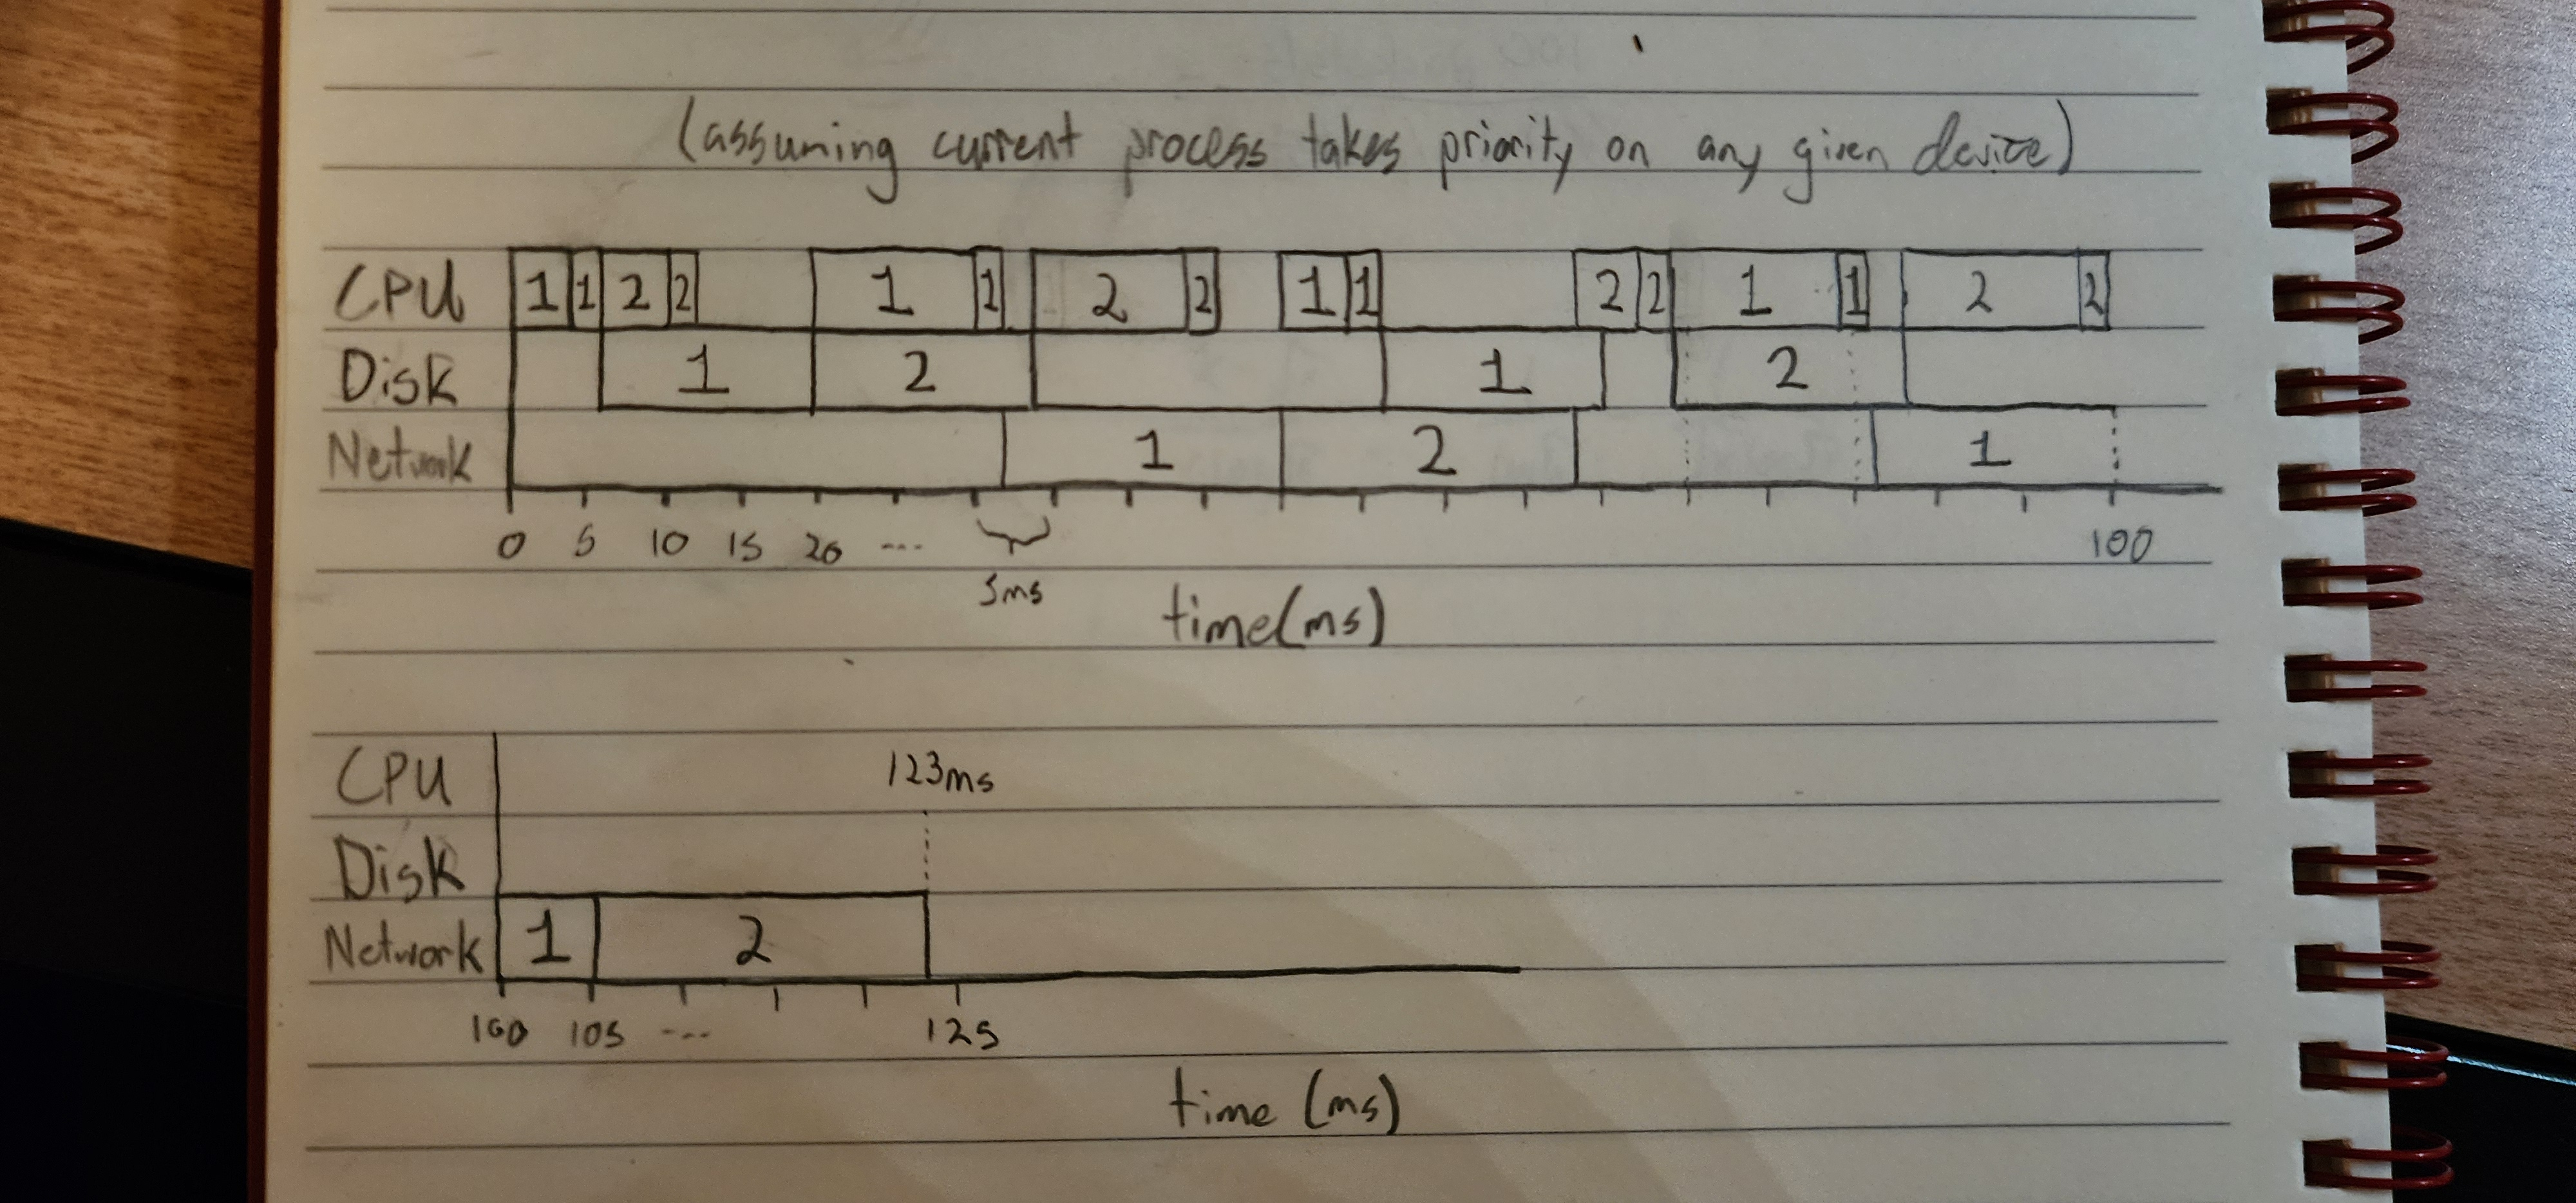
\includegraphics[width=5in]{3-3.jpg}
            \end{center}

            \pagebreak
            \item [d.)] Since it takes 123ms for both processes to iterate twice,
            we can see that the average utilization of each device is
            \[
                U_{\text{CPU}}
                = \frac{2(4 + 2 + 4 + 2 + 10 + 2 + 10 + 2)}{123}
                = \frac{72}{123}
                \approx 58\%
            \]
            \[
                U_{\text{Disk}}
                = \frac{2(14 + 14)}{123}
                = \frac{56}{123}
                \approx 45\%
            \]
            \[
                U_{\text{Network}}
                = \frac{2(18 + 18)}{123}
                = \frac{72}{123}
                \approx 58\%
            \]
        \end{itemize}

        \item [4.)] \begin{itemize}
            \item [a.)] We can run processes A and C simulataneously, as well
            as processes B and D, thus it takes 20 minutes for all of the
            processes to finish.

            \item [b.)] \
            \begin{center}
                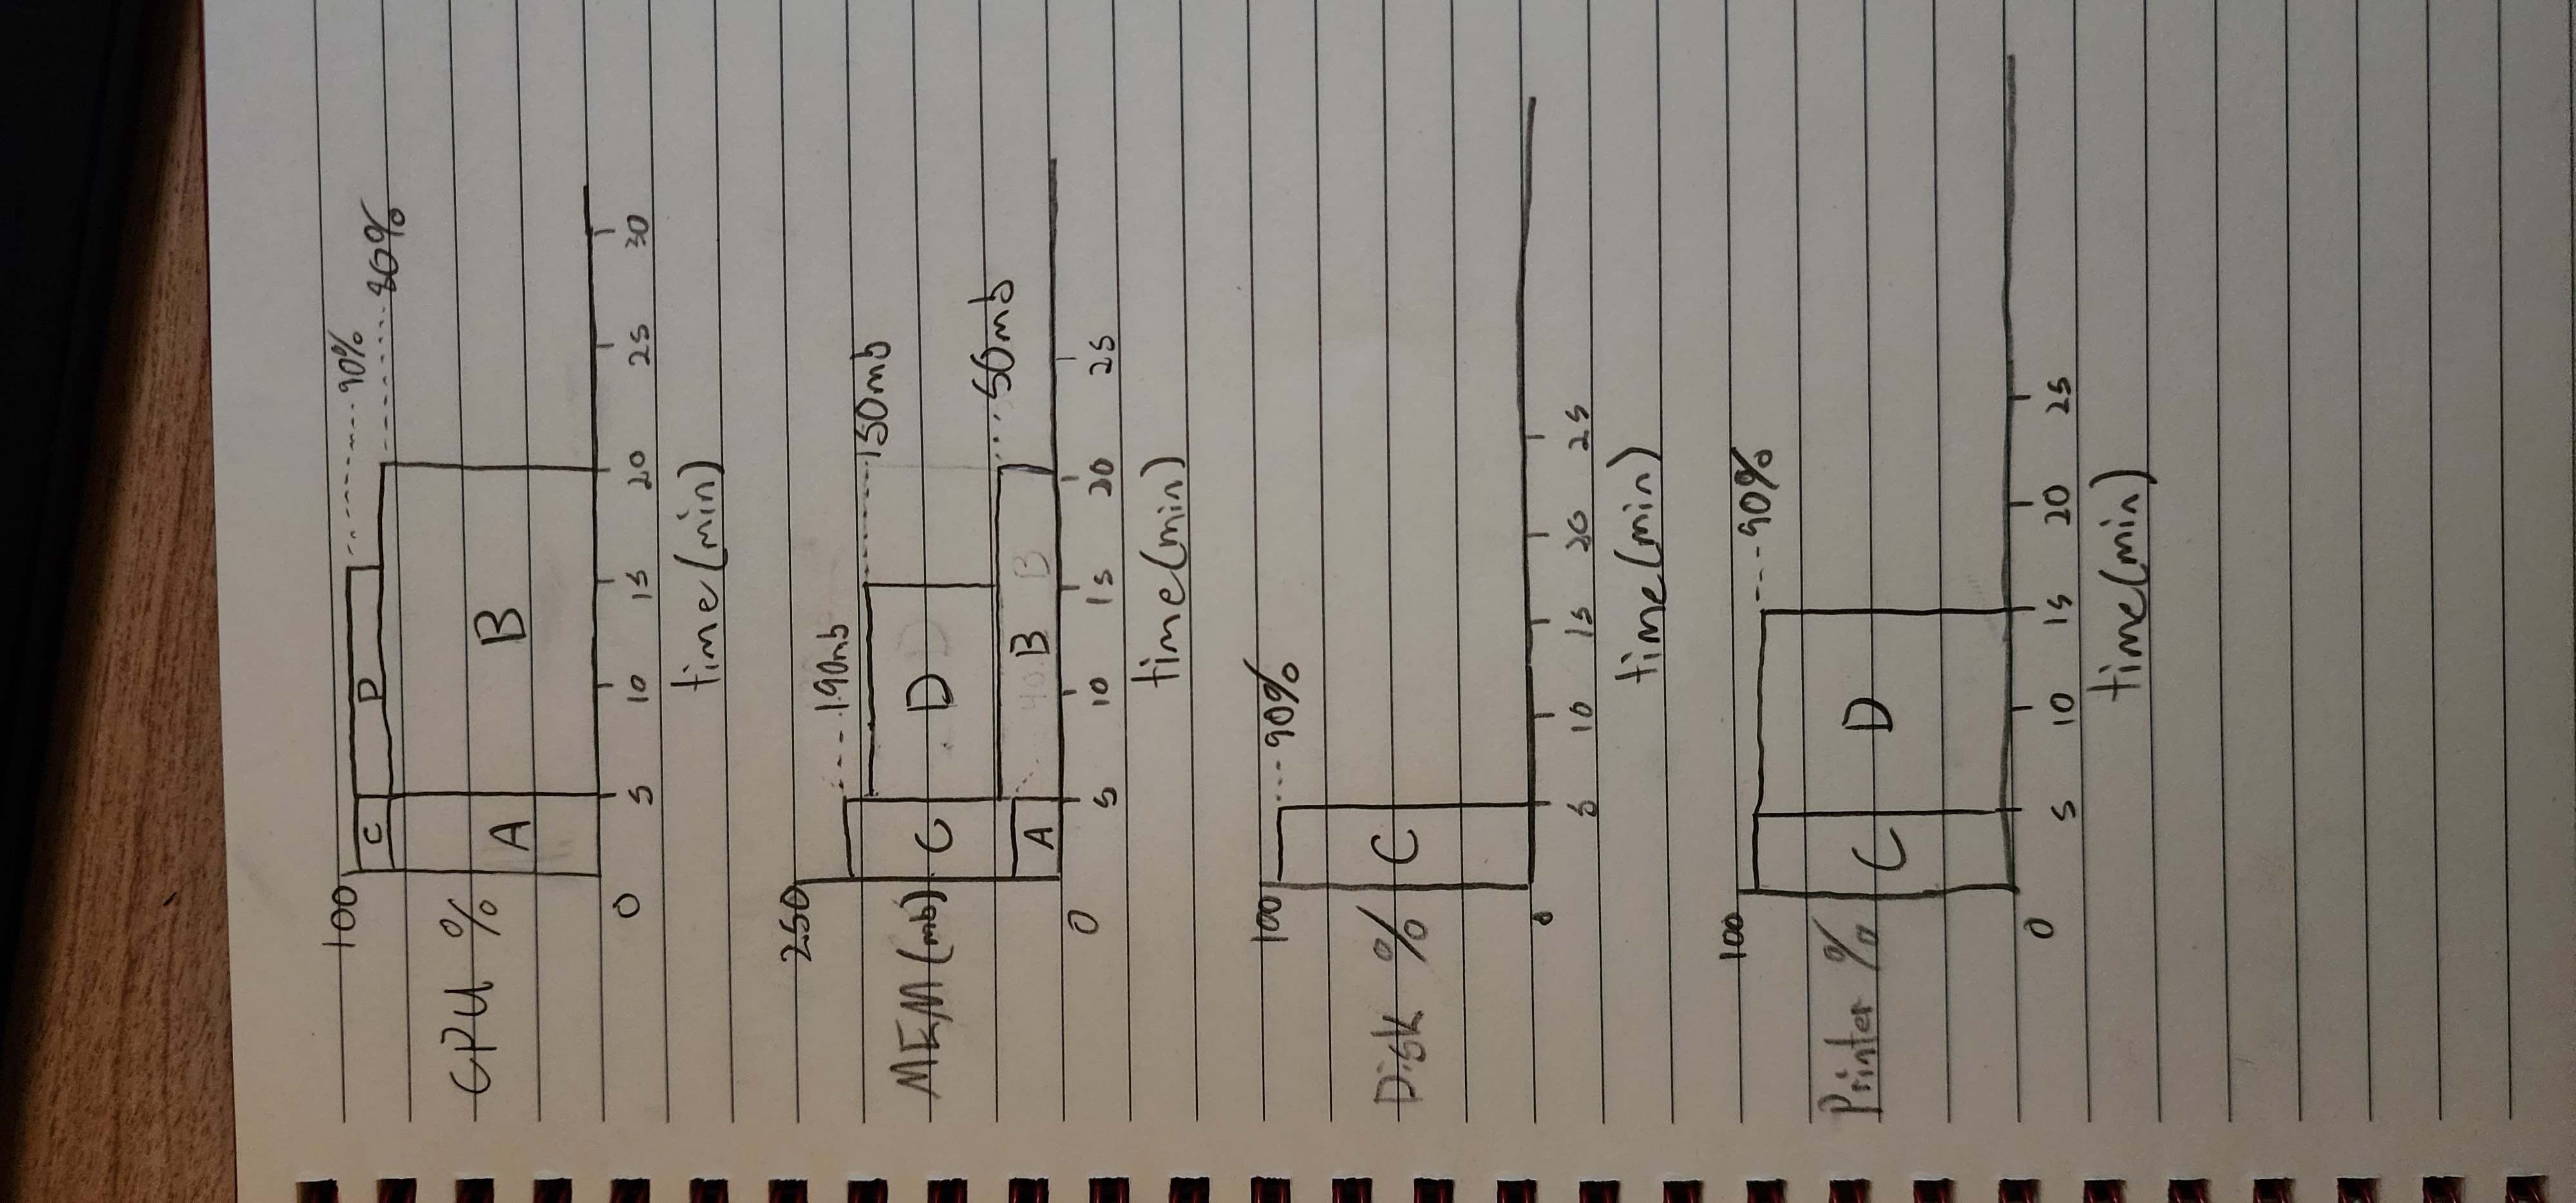
\includegraphics[height=3in, angle=-90]{4-2.jpg}
            \end{center}

            \item [c.)] The average utilization of each device is
            \[
                U_{\text{CPU}}
                = \frac{0.9 \times 15 + 0.8 \times 5}{20}
                = \frac{17.5}{20}
                = 87.5\%
            \]
            \[
                U_{\text{MEM}}
                = \frac{0.76 \times 5 + 0.6 \times 10 + 0.2 \times 5}{20}
                = \frac{10.8}{20}
                = 54\%
            \]
            \[
                U_{\text{Disk}}
                = \frac{0.9 \times 5}{5}
                = 90\%
            \]
            \[
                U_{\text{Printer}}
                = \frac{0.9 \times 15}{15}
                = 90\%
            \]

            \item [d.)] Four processes are completed in 20 minutes, so the
            average throughput is \\ 12 processes/hour.

            \item [e.)] The average turnaround time is
            \[
                T
                = \frac{5 + 5 + 10 + 15}{20}
                = \frac{35}{4}
                = 8.75\ \text{minutes}
            \]
        \end{itemize}

        \item [5.)] \begin{itemize}
            \item [a.)] Simply using ``\verb|top|'', and looking at the
            ``\verb|MiB Mem|'' row, we find that 11.2GiB of memory is available
            out of 15.7GiB total, thus the total memory utilization is
            $1 - (11.2 \div 15.7) = 1 - 0.71 = 0.29 = 29\%$.

            \item [b.)] Using ``\verb|$$|'' to get the process ID of the
            current command, we can run \\ ``\verb|pstree -s $$|'', which
            outputs \\
            ``\verb|systemd - sshd - sshd - sshd - bash - pstree|.''

            \item [c.)] Running ``\verb|ps -U root|'' lists every process
            belonging to the root user.
            To count the processes, run ``\verb=ps -U root | wc -l=''.
            In my case, the number was 161.

            \item [d.)] You can use ``\verb|uptime|''.
            In my case, the server has been up for 9 days and 32 minutes.
        \end{itemize}

        \item [6.)] \begin{verbatim}
            #include <stdio.h>
            #include <stdlib.h>
            #include <sys/wait.h>
            #include <unistd.h>

            int main(int argc, char** args) {
                fork();
                wait(NULL);
                printf("Process ID: %d\n", getpid());
                exit(0);

                return 0;
            }
        \end{verbatim}
    \end{itemize}
\end{document}